%%%%%%%%%%%%%%%%%%%%% PACKAGE IMPORTS %%%%%%%%%%%%%%%%%%%%%
\documentclass[11pt]{article}
\usepackage{amsmath, amsfonts, amsthm, amssymb}
\usepackage{lmodern}
\usepackage{microtype}
\usepackage{fullpage}

\usepackage[x11names, rgb]{xcolor}
\usepackage{graphicx}
\usepackage{circuitikz}
\usetikzlibrary{decorations,arrows,shapes}

\usepackage{etoolbox}
\usepackage{enumerate}
\usepackage{enumitem}
\usepackage{listings}
\usepackage{array}
\usepackage{mathtools}

\usepackage{tabularx}
\usepackage{booktabs} % For professional looking tables
\usepackage{caption}

% Adds a period (like Figure 1. A figure) and also bolds the "Figure 1." part
\captionsetup{labelsep=period,labelfont=bf}

%%%%%%%%%%%%%%%%%%%%%%%% QUESTION # %%%%%%%%%%%%%%%%%%%%%%%% % This part helps
%number your questions and creates a    %% % new page with each question for the
%aesthetics.        %% % It also creates parts that helps you answer questions
%%% % To use do: \begin{question} ... \end{question}         %% % and:
%\begin{part} ... \end{part}                       %%
%%%%%%%%%%%%%%%%%%%%%%%%%%%%%%%%%%%%%%%%%%%%%%%%%%%%%%%%%%%%

%% Latex Proof Template %\begin{part} %\textbf{Give a formal symbolic proof of
%the following statement.}
%%$$
%%\forall x [[(\forall y P(x, y)) \BI Q(x)] \IMP [Q(x) \IMP \exists y P(x,
%%%y)]]
%%$$
 %%   \begin{align*} %       & 1.1 \hspace{0.5cm} \forall x [(\forall y P(x, y))
 %\BI Q(x)] && %%\text{[Assumption]} \\
 %%       & 1.2 \hspace{0.5cm} \text{Let $a$ be arbitrary.} && \text{} \\
 %%       & 1.3 \hspace{0.5cm} (\forall y P(a, y)) \BI Q(a) && \text{[Eliminate
 %$\forall$ (1.1)]} \\
 %%       & 1.4 \hspace{0.5cm} P(a, b) \BI Q(a) && \text{[Eliminate %%$\forall$
 %(1.3)]} \\
  %%      & 1.5 \hspace{0.5cm} P(a, b) \IMP Q(a) \AND Q(a) \IMP P(a, b) &&
  %%%\text{[Definition of $\BI$ (1.4)]} \\
  %%      & 1.6 \hspace{0.5cm} Q(a) \IMP P(a, b) && \text{[Eliminate $\AND$
  %(1.5)]} \\
  %%      & 1.7 \hspace{0.5cm} Q(a) \IMP \exists y P(a, y) && \text{[Introduce
  %$\exists$ (1.6)]} \\
  %%      & 1.8 \hspace{0.5cm} \forall x[Q(x) \IMP \exists y P(x, y)] &&
  %%%\text{[Introduce $\forall$ (1.7)]} \\
    %%    2 \hspace{0.5cm} & \forall x [(\forall y P(x, y)) \BI Q(x)] \IMP
    %\forall x[Q(x) \IMP \exists y P(x, y)] && \text{[Direct Proof Rule (1.1 -
    %1.8)]}
   %% \end{align*}
%%
\setlength{\parindent}{0pt}
\setlength{\parskip}{5pt plus 1pt}

\newcommand{\mat}[1]{\textbf{#1}}

\providetoggle{questionnumbers}
\settoggle{questionnumbers}{true}
\newcommand{\noquestionnumbers}{
    \settoggle{questionnumbers}{false}
}

\newcounter{questionCounter}
\newenvironment{question}[2][\arabic{questionCounter}]{%
    \addtocounter{questionCounter}{1}%
    \ifnum\value{questionCounter}=1 {} \else {\newpage}\fi%
    \setcounter{partCounter}{0}%
    \vspace{.25in} \hrule \vspace{0.5em}%
        \noindent{\bf \iftoggle{questionnumbers}{Question #1: }{}#2}%
    \vspace{0.8em} \hrule \vspace{.10in}%
}

\newcounter{partCounter}[questionCounter]
\renewenvironment{part}[1][\alph{partCounter}]{%
    \addtocounter{partCounter}{1}%
    \vspace{.10in}%
    \begin{indented}%
       {\bf (#1)} %
}{\end{indented}}

\def\indented#1{\list{}{}\item[]} \let\indented=\endlist
\def\show#1{\ifdefempty{#1}{}{#1\\}}

%%%%%%%%%%%%%%%%%%%%%%%% SHORT CUTS %%%%%%%%%%%%%%%%%%%%%%%% % This is just to
%improve your quality of life. Instead  %% % of having to type long things, you
%can type short      %% % things. Ex: \IMP instead of \rightarrow to get ->
%%%
%%%%%%%%%%%%%%%%%%%%%%%%%%%%%%%%%%%%%%%%%%%%%%%%%%%%%%%%%%%%

\def\IMP{\rightarrow} \def\AND{\wedge} \def\OR{\vee} \def\BI{\leftrightarrow}
\def\DIFF{\setminus} \def\SUB{\subseteq} \def\P{\mathbb{P}} \def\E{\mathbb{E}}
\def\N{\mathbb{N}} \def\R{\mathbb{R}} \def\V{\text{Var}}

\newcolumntype{C}{>{\centering\arraybackslash}m{1.5cm}}
\renewcommand\qedsymbol{$\blacksquare$}

%%%%%%%%%%%%%%%%%%%%%%%%%%% TITLE %%%%%%%%%%%%%%%%%%%%%%%%%% %This is shows the
%homework number, your name, your collaborators, and the day. If you'd prefer to
%not show your name, just comment out the "\maketitle" below.
%%%
%%%%%%%%%%%%%%%%%%%%%%%%%%%%%%%%%%%%%%%%%%%%%%%%%%%%%%%%%%%%

\title{\vspace{-2cm}CSE 447: Assignment 1\vspace{-0.3cm}} \author{Abosh
Upadhyaya \thanks{\textbf{Collaborators: ChatGPT}. ChatGPT helped by providing
debugging advice, as well as explaining how to use inheritance in Python (for
the \texttt{WordPieceTokenizer} which inherited from the
\texttt{BytePairTokenizer}). It also helped me with making the scatterplots
(using \texttt{matplotlib}) and formatting the \LaTeX$\;$in this document.}}

\date{\vspace{-0.3cm} January 26, 2024 \vspace{-1cm}}

%%%%%%%%%%%%%%%%%%%%%%%% WORK BELOW %%%%%%%%%%%%%%%%%%%%%%%%
\begin{document}
\maketitle

% QUESTION 1
\begin{question}{$n$-gram Language Models}
	
	\textbf{Part 1: $n$-gram Language Modeling \& Perplexity}
	
	\begin{part}
		{\textbf{Describe how you built your $n$-gram models. Provide graphs,
		tables, charts or other summary evidence to support any claims you make.}}
		
		I built my $n$-gram models using a class called \texttt{NGramModel} which
		has a couple fields and methods. The fields are:
		\begin{itemize}
			\item \texttt{n}: The $n$ in $n$-gram.
			\item \texttt{ngram\_counts}: A dictionary that maps $n$-grams to their
			      counts.
			\item \texttt{context\_counts}: A dictionary that maps contexts to their
			      counts.
			\item \texttt{vocabulary}: A set of all the words in the vocabulary.
			\item \texttt{smoothing\_constant}: The smoothing constant used for
			      Laplace smoothing. Defaults to $1$.
			\item \texttt{lambdas}: A list of the $\lambda$ values used for
			      interpolation (for the trigram model).
		\end{itemize}
		
		From here, implementing the methods wasn't that bad. I just went back to the
		slides and implemented the necessary methods to complete the training and
		prediction processes.
		
		To train the model, I first preprocessed the data. This entailed tokenizing
		it (naive whitespace tokenization) and adding $n - 1$ START tokens to each
		line and a STOP token to the end of each line. I also converted all the
		tokens that appeared less than $3$ times to UNK tokens.
		
		Then, I built \texttt{vocabulary} by iterating through each line and adding
		each token to the set, making sure to discard the START token.
		
		Finally, I updated the \texttt{ngram\_counts} and \texttt{context\_counts}
		dictionaries by iterating through each $n$-gram in each line, and updating
		the counts accordingly.
		
		To predict (and calculate the model perplexity), I first preprocessed the
		data that needed to be predicted. This entailed tokenizing it (the same
		procedure as before, except this time we only UNKify tokens that appear less
		than $3$ times in the \textit{training} data).
		
		Then, for each line, I iterated through each $n$-gram in the line and used
		the maximum likelihood estimate to calculate the probability of the $n$-gram
		given the context. I then took the log of this probability and added it to a
		running sum of the log probabilities of each $n$-gram in the line.
		
		If the user wanted to use Laplace smoothing (specified by the
		\texttt{use\_laplace\_smoothing} parameter), I simply added the
		\texttt{smoothing\_constant} to the numerator and the
		\texttt{smoothing\_constant} times the vocabulary size to the denominator.
		
		Finally, I returned the perplexity of the model by taking the exponent of
		the negative of the average log probability of each $n$-gram in the line.
		The average was calculated by dividing the total summed log probabilities
		for all sentences in the set divided by the total number of tokens in the
		set, making sure to subtract the amount of START tokens in each line, as
		they're not part of the vocabulary and our model can't predict them.
		
		Adding interpolation was not that bad. I simply added a new method called\\
		\texttt{perplexity\_with\_interpolation} which did almost exactly the same
		thing, except it also took a unigram and bigram model (to be used for
		interpolation). From there, I computed the average perplexity by doing the
		same thing as before except using the interpolation formula.
	\end{part}
	
	\begin{part}
		{\textbf{Describe how you computed \textit{perplexity} without any smoothing
		in a detailed equation, in natural language, or with pseudo code.}}
		
		As I stated in my answer to part (a), I returned the perplexity of the model
		by taking the exponent of the negative of the average log probability of
		each $n$-gram in the line. The average was calculated by dividing the total
		summed log probabilities for all sentences in the set divided by the total
		number of tokens in the set, making sure to subtract the amount of START
		tokens in each line, as they're not part of the vocabulary and our model
		can't predict them.
	\end{part}
	
	\begin{part}
		{\textbf{What’s the potential downside of Laplace smoothing? Back up your
		claim with empirical evidence.}}
		
		One potential downside of Laplace smoothing is that it might add too much
		probability mass to a rare event or $n$-gram. Which is kind of crazy,
		because it's only adding 1 to the count of each token. But, if you think
		about it, if you have a very large vocabulary, adding 1 to the count of each
		token will add a lot of probability mass to the rare or unseen tokens, which
		barely appear at all in the training data.
		
		Basically, because it's uniform, it adds too much probability mass to the
		rare events, which is not good.
		
		Here's some empirical evidence to show why this is bad. I analyzed the
		unigram, bigram, and trigram models with and without Laplace smoothing on
		\textbf{the training set}. Here were the results:
		    
		\begin{table}[ht]
			\centering
			\begin{tabular}{|l|l|l|}
				\hline
				\textbf{Model} & \textbf{No Smoothing} & \textbf{Laplace Smoothing
				($k=1.0$)} \\ \hline
				1-gram         & 976.54                & 977.50                    \\
				\hline
				2-gram         & 77.07                 & 1,442.30                  \\
				\hline
				3-gram         & 7.87                  & 6,244.42                  \\
				\hline
			\end{tabular}
			\caption{Perplexity scores of language models with and without Laplace
				smoothing ($k=1.0$)}
		\end{table}
		
		As can be seen, the perplexity of the models with Laplace smoothing is
		significantly higher than the perplexity of the models without Laplace
		smoothing \textbf{on the training set}.
	\end{part}
	
	\vspace{1.5cm}
	
	\begin{part}
		{\textbf{Another extension of Laplace smoothing, instead of adding $1$ to
			the count of each token, is to add $k$, where typically $0 < k < 1$. Try
			different values for $k$, and describe how different $k$ change the
			perplexity score differently.}}
		
		I ran the same experiment, except this time with a smoothing constant of $k
		= 0.001$. Here were the results:
		\begin{table}[ht]
			\centering
			\begin{tabular}{|l|l|l|}
				\hline
				\textbf{Model} & \textbf{No Smoothing} & \textbf{Laplace Smoothing
				($k=0.001$)} \\ \hline
				1-gram         & 976.54                & 976.54                    \\
				\hline
				2-gram         & 77.07                 & 95.08                     \\
				\hline
				3-gram         & 7.87                  & 35.09                     \\
				\hline
			\end{tabular}
			\caption{Perplexity scores of language models with and without Laplace
				smoothing ($k=0.001$)}
		\end{table}

		Of course, no smoothing is best on the training set as expected since our
		model was trained on the training set. But, as $k$ got smaller and smaller,
		the perplexity got smaller and smaller on the \textbf{training set}. This
		makes sense, because as $k$ gets smaller and smaller, the amount of
		probability mass added to each token gets smaller and smaller, which is
		better for the model.
		
		However, on the dev and test sets, the happy medium was not just to move $k$
		closer and closer to $0$. In fact, the best $k$ for the dev set was
		somewhere around $0.03$ (although I didn't rigorously test this, I just
		plugged some values in and saw the best one, so maybe there's a better
		one.).
	\end{part}
	
	\begin{part}
		{\textbf{Report the \textit{unsmoothed} and \textit{smoothed with Laplace
			smoothing} version of perplexity scores of the unigram, bigram, and
			trigram language models for your training, development, and test sets.
			Briefly discuss the experimental results.}}
		
		Here are the results:
		\begin{table}[ht]
			\centering
			\begin{tabular}{|l|l|l|}
				\hline
				\textbf{Model}    & \textbf{No Smoothing} & \textbf{Laplace Smoothing
				($k=1.0$)} \\ \hline
				1-gram (Training) & 976.54                & 977.51                    \\
				\hline
				2-gram (Training) & 77.07                 & 1,442.30                  \\
				\hline
				3-gram (Training) & 7.87                  & 6,244.42                  \\
				\hline
				1-gram (Dev)      & 892.24                & 894.39                    \\
				\hline
				2-gram (Dev)      & $\infty$              & 1,669.65                  \\
				\hline
				3-gram (Dev)      & $\infty$              & 9,676.65                  \\
				\hline
				1-gram (Test)     & 896.49                & 898.55                    \\
				\hline
				2-gram (Test)     & $\infty$              & 1,665.38                  \\
				\hline
				3-gram (Test)     & $\infty$              & 9,649.60                  \\
				\hline
			\end{tabular}
			\caption{Perplexity scores of language models with and without Laplace
			smoothing ($k=1.0$)}
		\end{table}
		
		
		It is expected that the model had infinite perplexity on the dev and test
		sets. This is because the model was trained on the training set, and the dev
		and test sets might contain n-grams that were never seen in the training
		sets. Thus, the model would assign a probability of $0$ to these n-grams,
		and the perplexity would be infinite.
		
		It's also interesting to see the perplexity be so high for $k = 1.0$. As I
		said in my answer to part (d), if we change $k$ to be something like $0.03$,
		these are the results:
		
		\begin{table}[ht]
			\centering
			\begin{tabular}{|l|l|l|}
				\hline
				\textbf{Model}    & \textbf{No Smoothing} & \textbf{Laplace Smoothing
				($k=0.03$)} \\ \hline
				1-gram (Training) & 976.54                & 976.54                    \\
				\hline
				2-gram (Training) & 77.07                 & 235.46                    \\
				\hline
				3-gram (Training) & 7.87                  & 409.10                    \\
				\hline
				1-gram (Dev)      & 892.25                & 892.29                    \\
				\hline
				2-gram (Dev)      & $\infty$              & 521.28                    \\
				\hline
				3-gram (Dev)      & $\infty$              & 3,567.91                  \\
				\hline
				1-gram (Test)     & 896.50                & 896.54                    \\
				\hline
				2-gram (Test)     & $\infty$              & 519.04                    \\
				\hline
				3-gram (Test)     & $\infty$              & 3,549.07                  \\
				\hline
			\end{tabular}
			\caption{Perplexity scores of language models with and without Laplace smoothing ($k=0.03$)}
		\end{table}
		
		Notice how now, the perplexity for the bigram model is much lower than the
		perplexity for the unigram model! This could be because of the data of
		course, but it was an interesting result.
		
	\end{part}
	
	
	\begin{part}
		{\textbf{Your goal is to find reasonably good combinations of $\lambda_1$,
			$\lambda_2$, $\lambda_3$. Experiment and report perplexity scores on
			training and development sets for five sets of values of $\lambda_1$,
			$\lambda_2$, $\lambda_3$ that you tried, along with short descriptions of
			the strategies that you used to find better hyperparameters. In addition,
			report the training and development perplexity for the values $\lambda_1 =
			0.1, \lambda_2 = 0.3, \lambda_3 = 0.6$.}}
		
		Here are the results of running grid search to find the best $\lambda$
		values for interpolation on the training and dev sets:
		
		\begin{table}[ht]
			\centering
			\begin{tabular}{|l|l|l|}
				\hline
				\textbf{$\lambda$ values} & \textbf{Training Perplexity} & \textbf{Dev     
				Perplexity} \\ \hline
				(0.1, 0.1, 0.8)           & 9.33                         & 482.85 \\
				\hline
				\textbf{(0.1, 0.3, 0.6)}  & \textbf{11.15}               &
				\textbf{352.23} \\ \hline
				(0.1, 0.5, 0.4)           & 14.17                        & 308.64 \\
				\hline
				(0.3, 0.1, 0.6)           & 11.97                        & 364.09 \\
				\hline
				(0.3, 0.3, 0.4)           & 15.30                        & 286.63 \\
				\hline
				(0.3, 0.5, 0.2)           & 22.44                        & 262.89 \\
				\hline
				(0.5, 0.1, 0.4)           & 16.82                        & 334.72 \\
				\hline
				(0.5, 0.3, 0.2)           & 25.06                        & 280.50 \\
				\hline
			\end{tabular}
			\caption{Perplexity scores for different $\lambda$ values on an
      interpolated trigram model}
		\end{table}

    I determined the optimal hyperparameters with a standard grid search. I
    tried a bunch of different combinations of $\lambda$ values that summed to
    1, and printed their perplexity scores on the training and dev sets. I then
    picked the $\lambda$ values that had the lowest perplexity on the dev set.
	\end{part}
	
	\vspace{3.5cm}
	
	\begin{part}{\textbf{Putting it all together, report perplexity on the test
			set, using the best combination of hyperparameters that you chose from the
			development set. Specify those hyperparameters.}}
		
		\begin{table}[ht]
			\centering
			\begin{tabular}{|l|l|}
				\hline
				\textbf{$\lambda$ values} & \textbf{Test Perplexity} \\ \hline
				(0.3, 0.5, 0.2)           & 262.66                   \\ \hline
			\end{tabular}
			\caption{Perplexity for the best $\lambda$ values on an interpolated trigram model}
		\end{table}
		
	\end{part}
	
	\begin{part}{\textbf{If you use half of the training data, would it increase
			or decrease the perplexity of previously unseen data? Why? Provide
			empirical experimental evidence to support your claims.}}
		
		It will increase the perplexity of previously unseen data. This is because
		the model will be trained on less data, so it will be less accurate. This
		will cause the perplexity to increase, as the model has less of an "idea" of  
		what words could come next. This means it has to store more information each
		time it predicts a word, which means the perplexity will increase.
		
		When I trained the interpolated model on half of the training data, here
		were the results:
		
		\begin{table}[ht]
			\centering
			\begin{tabular}{|l|l|l|}
				\hline
				\textbf{$\lambda$ values} & \textbf{Dev Perplexity} & \textbf{Test
				Perplexity} \\ \hline
				(0.1, 0.1, 0.8)           & $\infty$                & $\infty$     \\
				\hline
				(0.1, 0.3, 0.6)           & $\infty$                & $\infty$     \\
				\hline
				(0.1, 0.5, 0.4)           & $\infty$                & $\infty$     \\
				\hline
				(0.3, 0.1, 0.6)           & $\infty$                & $\infty$     \\
				\hline
				(0.3, 0.3, 0.4)           & $\infty$                & $\infty$     \\
				\hline
				(0.3, 0.5, 0.2)           & $\infty$                & $\infty$     \\
				\hline
				(0.5, 0.1, 0.4)           & $\infty$                & $\infty$     \\
				\hline
				(0.5, 0.3, 0.2)           & $\infty$                & $\infty$     \\
				\hline
			\end{tabular}
			\caption{Perplexity scores for different $\lambda$ values on the dev and test sets }
		\end{table}
		
		The perplexities on both the dev and test sets became $\infty$. The only way
		this can happen is if the model had an interpolated probability of $0$ for
		some $n$-gram in the dev or test set. That means it encountered some unseen
		token in the dev or test set, which is more likely now that we only trained
		the model on half of the training data.
		
		Normally (in this assignment), at least the unigram model will have a
		non-zero probability for an $n$-gram since all individual tokens in the dev
		and test set are in the training set, but because there's no smoothing with
		the interpolated model, a single unseen token will cause the interpolated
		probability to be $0$, which will cause the perplexity to be $\infty$. And
		since we only trained on half the training data, there were some unseen
		tokens.
	\end{part}
	
	\vspace{2.5cm}
	
	\begin{part}{\textbf{If you convert all tokens that appeared less than five
			times to ⟨unk⟩ (a special symbol for out-of-vocabulary tokens), would it
			increase or decrease the perplexity on the previously unseen data compared
			to an approach that converts only those words that appeared just once to
			⟨unk⟩? Why? Provide empirical evidence to support your claims.}}
		
		Converting all tokens that appear less than 5 times to ⟨UNK⟩ will decrease
		the perplexity on the previously unseen data compared to an approach that
		converts only those words that appeared just 1 to ⟨UNK⟩.
		
		Here are the results after testing different $\lambda$ values on the dev and
		test sets with different ⟨UNK⟩ thresholds:
		
		\begin{table}[ht]
			\centering
			\begin{tabular}{|l|l|l|l|l|}
				\hline
				\textbf{$\lambda$ values} & \textbf{Dev ($= 1$)} & \textbf{Dev ($< 5$)}
				& \textbf{Test ($= 1$)} & \textbf{Test ($< 5$)} \\ \hline
				(0.1, 0.1, 0.8) & $559.92$ & 391.15 & $555.84$ & 389.67 \\ \hline
				(0.1, 0.3, 0.6) & $406.70$ & 287.70 & $403.94$ & 286.85 \\ \hline
				(0.1, 0.5, 0.4) & $355.51$ & 253.19 & $353.33$ & 252.64 \\ \hline
				(0.3, 0.1, 0.6) & $415.13$ & 302.13 & $413.20$ & 301.48 \\ \hline
				(0.3, 0.3, 0.4) & $325.14$ & 239.99 & $323.75$ & 239.63 \\ \hline
				(0.3, 0.5, 0.2) & $297.28$ & 221.23 & $296.22$ & 221.11 \\ \hline
				(0.5, 0.1, 0.4) & $378.09$ & 281.50 & $377.00$ & 281.24 \\ \hline
				(0.5, 0.3, 0.2) & $315.07$ & 238.08 & $314.33$ & 238.09 \\ \hline
			\end{tabular}
			
			\caption{Perplexity scores for different $\lambda$ values with different ⟨UNK⟩ thresholds}
		\end{table}
		
		This decrease in perplexity is probably because the model is dealing with a
		smaller, more generalized vocabulary. In other words, the model is better at
		handling unseen data when it generalizes words that don't appear frequently
		into the ⟨UNK⟩ token, rather than treating them as individual tokens. This
		generalization probably allows the model to use its learned probabilities
		more effectively because it isn't distracted by the noise of rare words,
		which it hasn't learned meaningful information about during training.
	\end{part}
	
\end{question}

\begin{question}{Byte-Pair Encoding}
	
	\begin{part}{\textbf{Please produce a scatterplot showing points $(x,y)$, each
			corresponding to an iteration of the algorithm, with $x$ the current size
			of the type vocabulary (including the base vocabulary), and $y$ the length
			of the training corpus (in tokens) under that vocabulary’s types. How many
			types do you end up with? What is the length of the training data under
			your final type vocabulary?}}
		
		\begin{figure}[ht]
			\centering
			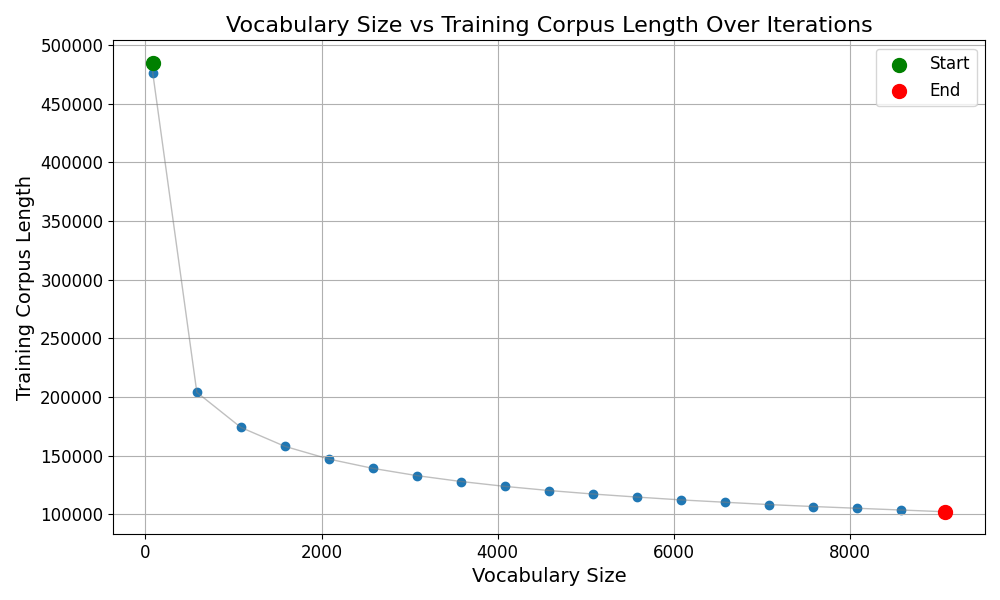
\includegraphics[width=\textwidth]{bpe_training.png}
			\caption{Scatterplot of training corpus length (in tokens) ($y$-axis)
				versus vocabulary size ($x$-axis). Each point represents the state at
				every $\mathbf{500}$th iteration of the BPE training algorithm.}
		\end{figure}
		
		The final vocabulary size was $\boxed{9,219}$ types. The number of tokens in
		the training corpus after termination was $\boxed{101,849}$.
	\end{part}

  \vspace{4cm}
	
	\begin{part}{\textbf{Another way of overcoming the rare word issue is to
			encode text as a sequence of characters. Discuss the advantages and
			potential issues of character-level encoding compared to BPE.}}
		
		\begin{table}[ht]
			\centering
			\begin{tabularx}{\textwidth}{|X|X|}
				\hline
				\textbf{Advantages over BPE}                                       &
				\textbf{Disadvantages to BPE} \\
				\hline
				\textbf{This is a much simpler algorithm to implement.} It's just a
				simple loop that iterates through each character in the training data
				and adds it to the vocabulary. This is much simpler than the BPE
				algorithm, which can be really complicated to implement and debug. &                               
				Because we're encoding each character, the length of a sequence the
				model has to process is \textbf{much longer}. This leads to worse
				performance and efficiency. BPE however, can encode a sequence of
				characters as a single token, which is much more efficient. \\
				\hline
				\textbf{There is no need to worry about out-of-vocabulary words}, since
				we are essentially encoding every single possible character in the
				language. Thus, our model can represent any text, regardless of whether
				it's in the training data or not. BPE on the other hand, can only
				represent tokens that are in the training data, so there's still a
				possibility of encountering an out-of-vocabulary token.            &
				Linguistically speaking, there is a benefit in storing tokens that that
				aren't just characters. This is because words have \textbf{meaning}, and
				encoding them as individual characters can lose that meaning. For
				example, the suffix ``ing" is a common suffix in English that denotes
				the present participle tense. If we encode each character as a token, we
				lose this meaning, and the model has to learn it from scratch. BPE
				allows us to retain this meaning, as it can encode the suffix ``ing" as
				a single token. \\
				\hline
			\end{tabularx}
      \caption{Advantages and disadvantages of character-level encoding compared
      to BPE.}
		\end{table}
		
	\end{part}
	
	\begin{part}{\textbf{Applying your tokenizer on the last $1000$ lines of the
			data, how many tokens do you end up with? Do you encounter issues with
			words that didn’t appear in the training set? More generally, when would
			you expect your tokenizer to fail when applying to an unseen text.}}
		
		I ended up with $\boxed{27,969}$ tokens. I did not encounter any issues with
		words that didn't appear in the training set. I'm guessing this is because
		the training and test sets are from the same language distribution, so they
		are correlated well and the tokens BPE formed matched the test set well.
		
		However, in general, this is true of BPE anyways. BPE picks up on linguistic
		patterns inside of words themselves and forms tokens based on those
		patterns. But, there are obviously cases where BPE can fail.
		
		An easy example is if the training data is not representative of the
		language patterns in the test set or in the real world (depending on your
		model's use case). For example, if the training data is from a different
		language distribution than the test set, then BPE will fail because it will
		form tokens based on the training data, which will not match the test set.
		It'd be like teaching someone to speak in a certain dialect which is
		region-specific, and then asking them to try and predict what someone who
		was from a completely different part of the world would say. They'd have no
		knowledge of the language patterns in that region, so they'd do a bad job
		even if they understood their dialect well.
	\end{part}
	  
\end{question}

\begin{question}{\texttt{WordPiece}}
	
	\begin{part}{\textbf{Please produce a scatterplot showing points $(x,y)$, each
			corresponding to an iteration of the algorithm, with $x$ the current size
			of the type vocabulary (including the base vocabulary), and $y$ the length
			of the training corpus (in tokens) under that vocabulary’s types. How many
			types do you end up with? What is the length of the training data under
			your final type vocabulary?}}
		
		\begin{figure}[ht]
			\centering
			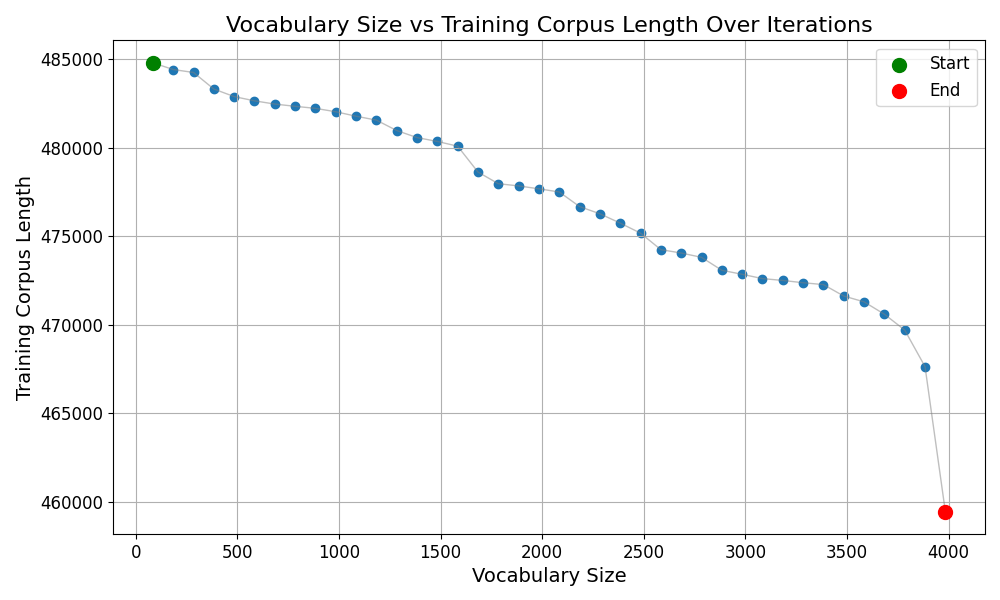
\includegraphics[width=\textwidth]{wordpiece_training.png}
			\caption{Scatterplot of training corpus length (in tokens) (y-axis) versus
				vocabulary siz (x-axis). Each point represents the state at every
				$\mathbf{100}$th iteration of the \texttt{WordPiece} training
				algorithm.}
		\end{figure}
		
		The final vocabulary size was $\boxed{4,083}$ types. The number of tokens in
		the training corpus after termination was $\boxed{455,238}$ (hey, less
		tokens means we merged more!).
		
	\end{part}
	
	\begin{part}{\textbf{Applying your tokenizer on the last $1000$ lines of the
			data, report the length of the tokenized data. Also, include the tokenized
			sequences for the following two sentences:}}
		
		The length of the tokenized data in tokens was $\boxed{108,692}$ tokens.
		
		\begin{enumerate}[label=\roman*)]
			\item \textit{``Analysts were expecting the opposite, a deepening of the
			deficit."}
			
			[`A', `n', `a', `l', `y', `s', `t', `s', `Ġ', \\`w', `e', `r', `e', `Ġ',\\
				`exp', `e', `c', `t', `i', `n', `g', `Ġ', \\`th', `e', `Ġ', \\`o', `p',
				`p', `o', `s', `i', `t', `e', `,', `Ġ', \\`a', `Ġ', \\`d', `e', `e',
				`p', `e', `n', `i', `n', `g', `Ġ', \\`o', `f', `Ġ', \\`d', `e', `f',
				`i', `c', `i', `t', `.']
			      
			\item \textit{``Five minutes later, a second person arrived, aged around
			thirty, with knife wounds."}
			
			[`F', `i', `v', `e', `Ġ', \\`m', `i', `n', `u', `t', `e', `s', `Ġ', \\`l',
				`a', `t', `e', `r', `,', `Ġ',\\ `a', `Ġ', \\`s', `e', `c', `o', `n',
				`d', `Ġ', \\`p', `e', `r', `s', `o', `n', `Ġ', \\`a', `r', `r', `i',
				`v', `e', `d', `,','Ġ', \\`a', `g', `e', `d', `Ġ', \\`a', `r', `o', `u',
				`n', `d', `Ġ', \\`th', `i', `r', `t', `y', `,','Ġ', \\`w', `i', `th',
				`Ġ', \\`k', `n', `i', `f', `e', `Ġ', \\`w', `o', `u', `n', `d', `s',
				`.',']
		\end{enumerate}
	\end{part}
	
	\vspace{12cm}
	
	\begin{part}{\textbf{In terms of efficiency and performance, what’s the
			advantages and disadvantages of \texttt{WordPiece} compared with BPE?
			There is no single correct answer here, just provide your thoughts and
			rationales, supported by empirical evidences.}}
		\begin{table}[ht]
			\centering
			\begin{tabularx}{\textwidth}{|X|X|}
				\hline
				\textbf{Advantages over BPE} & \textbf{Disadvantages to BPE} \\
				\hline
				\texttt{WordPiece} normalizes the frequency of the two adjacent tokens
				by their relative frequencies. For example, if the tokens "Hi there"
				appear 100 times together in the training set, much higher than any
				other adjacent tokens, BPE would immediately merge them together as a
				token and move forward. Meanwhile, if the tokens ``Calif" and ``ornia"
				appear only 5 times together in the training set, BPE would skip them on
				this iteration (and likely) continue to skip them for many iterations,
				since they're not frequently occurring together. However,
				\texttt{WordPiece} would note that yes, they don't appear together
				often, but they almost only appear \textit{together}. That is, you never
				see ``Calif" or ``ornia" by itself, and you do see them together, which
				implies they should be merged. So \texttt{WordPiece} picks up on these
				linguistic patterns and merges them together, which is a huge advantage.
				& BPE is simpler to understand than \texttt{WordPiece}. The tokenization
				algorithm for \texttt{WordPiece} can also be difficult, since we're
				searching for the longest matching subword, instead of just merging
				tokens until we can't merge them anymore! Additionally, the optimization
				criteria for BPE is simple: simply choose the most frequently occuring
				pair of adjacent tokens and merge them. \texttt{WordPiece} is a bit more
				complex, and furthermore, requires more calculations as we have to not
				only calculate the frequency of the pair of tokens but also the
				frequency of each token individually. This makes it more computationally
				expensive than BPE. \\
				\hline
			\end{tabularx}
      \caption{Advantages and disadvantages of \texttt{WordPiece} compared to
      BPE.}
		\end{table}

		In terms of \textbf{empirical evidence}, if we look at the two graphs, it
		isn't directly clear which one is better. Sure, they both decrease the size
		of the training corpus as they merge tokens together, but we can't just
		compare the size of the test corpus to determine which one is better,
		because we had different training criterion.

		Perhaps the $\log$ scale of the BPE graph is because we trained for too
		long, and after a while, it becomes harder and harder to minimize the size
		of the training corpus. And perhaps we trained the \texttt{WordPiece} model
		for too short of a time, and if we trained it for longer, we'd see that
		sharp decrease at the end for even longer at the end of the graph.

		In BPE, we stopped when the frequency of the next most frequent pair was 2.
		In WordPiece, we just learned 4,000 merge rules and stopped. So it's not
		fair to compare these models as is.

		However, I do know about WordPiece's usage with BERT, and I know that it
		performs well with masked-language modeling (where you mask out a word and
		try to predict it). BPE might excel at tasks that require more common
		phrases, as it can more efficiently encode them, but I think that WordPiece
		would perform similarly as well, as it's also still directly correlated to
		the frequency of the tokens appearing together! In a sense, WordPiece is
		just a level up from BPE, as it's more sophisticated and requires more
		calculations, but it's still based on the same idea of merging tokens
		together based on their frequency of occurrence.
	\end{part}
\end{question}
\end{document}